\documentclass[twocolumn]{article}
\usepackage{indentfirst}
\usepackage{graphicx}
\usepackage{microtype}
\usepackage{algorithm}
\usepackage{algpseudocode}
\usepackage{lmodern}
\usepackage{ragged2e}
\usepackage{amsmath}
\usepackage{float}
\usepackage{hyperref}





\title{Using CNN to assist Dermatologist to detect cancer in Ghana}
\author{Derry Emmanuel : PS/MCS/22/0012}
\date{}
\begin{document}
\maketitle
\raggedbottom
\begin{abstract}
Skin cancer is one of the most common types of cancer worldwide.  Skin cancers are caused by different factors, such as prolonged exposure to sunlight, environmental factors, and genetic defects. This can be mainly divided into benign and malignant. Although skin cancer is a threat to human life, fortunately, early detection could be critical for successful treatment and improved prognosis. Image processing techniques have been increasingly used in the healthcare industry to assist in detecting and diagnosing various skin diseases. In this paper, I will explore the use of image processing techniques for the automated detection of skin cancer leveraging a Convolutional Neural Network. The proposed approach involves preprocessing of the skin lesion images followed by feature extraction and classification. The preprocessing step involves noise removal and enhancement of the image through rotation, zooming, and other operations.  The features are then extracted from the images using texture analysis techniques such as gray-level co-occurrence matrix (GLCM) and local binary pattern (LBP). Finally, a classifier is trained on the extracted features to classify the images into any of the skin cancer classes stated in section two of this paper. In evaluating the proposed approach, a dataset of skin lesion images from the International Skin Imaging Collaboration (ISIC) is used. The results show that the proposed approach achieves an accuracy of 87.5\% in classifying the skin lesion images into one of the nine skin cancer classes. This suggests that image-processing techniques can be used effectively for the automated detection of skin cancer and it can further be enhanced using Machine Learning models.
\end{abstract}
\section{Introduction}
Skin cancer is one of the most common types of cancer worldwide. According to the American Cancer Society, skin cancer accounts for approximately 5.4 million cases in the United States alone. Presently, dermatologists' visual inspection is the most common method used for skin cancer diagnosis. However, this method is subjective and relies on the experience of the dermatologist. Moreover, it can be time-consuming and costly, especially in areas where access to dermatologists is limited. According to research conducted the curable rate will be more than 90\% high if cancer can be diagnosed in its early stages while the curable rate will be less than 50\% in its later stage. With respect to this research, the detection of skin cancer in the early stages has been considered a vital issue, and Computer Aided Diagnosis is an important tool for this. Results show that the proposed approach achieves an accuracy of 87.5\% in classifying the skin lesion images into one of the nine skin cancer classes. This suggests that image-processing techniques can be used effectively for the automated detection of skin cancer and it can further be enhanced using Machine Learning models.
\section{Literature Review}
According to studies, CNNs are capable of categorizing skin lesions with dermatologist-level precision, which could result in quicker and more accurate diagnosis. Despite ongoing difficulties, the development and application of CNNs in dermatology hold promise for bettering patient outcomes and the detection of skin cancer.\cite{esteva2017dermatologist} showed the potential of CNNs in skin cancer detection by creating a deep-learning model that classified skin lesions with dermatologist-level accuracy. A dataset of 129,450 clinical photos covering more than 2,000 disorders was used by the scientists to train their CNN. With a sensitivity of 96.3\% and a specificity of 90.3\% for melanoma diagnosis, the model performed admirably. The study proved that CNNs might be used to detect skin cancer and emphasized the potential of AI-based solutions to improve dermatologists' diagnostic abilities.
 In recent years, several strategies of automated computer image analysis have been investigated as an aid for physicians to provide high and widely reproducible diagnostic accuracy for skin screening \cite{haenssle2018man}.. The awareness of the biomedical technical public for computer-maintained dermoscopic pictures of skin inspection and characterization has increased through the past years. Diagnosis of malicious malignancy is laborious since other skin injuries can have similar physical physiognomies \cite{deshpande2016automated}. In a study on the classification of pigmented skin lesions, \cite{tschandl2019comparison} compared the diagnostic precision of four machine-learning algorithms, including a CNN, with that of human readers (dermatologists, residents, and medical students). According to the study, CNN was more sensitive and specific than human readers at detecting melanoma. This study provided more evidence in favor of CNNs' potential to help dermatologists identify skin cancer accurately.
Despite the promise that CNNs have shown in the detection of skin cancer, there are still a number of issues and restrictions that need to be resolved. The requirement for sizable, varied, and well-annotated training datasets \cite{han2018classification}; the possibility of biases in the data that could result in skewed predictions (Adamson \& Smith, 2018); and the interpretability and explainability of the CNN models \cite{holzinger2019causability} are a few of these.
Automated classification of skin cancer has been achieved through a variety of modalities, such as Raman spectroscopy, optical coherence tomography, and electrical impedance. However, the simplest modality is digital photography, often enhanced by a dermatoscopy. Given the near ubiquitous use of digital cameras and dermatoscopic in dermatologic practice, digital image-based ML models have the greatest potential for clinical implementation and are thus the focus of this term paper. 
Image processing techniques can be used to extract features from medical images that are not visible to the naked eye. These features can be used to train a classifier that can automatically classify images into different classes. This can help reduce the subjectivity and time required for visual inspection by dermatologists.
In this paper, I intend to explore the use of image-processing techniques for the automated detection of skin cancer using a convolutional neural network. The proposed approach involves preprocessing of the skin lesion images followed by feature extraction and classification. The rest of the paper is organized as follows.  Section 2 describes the dataset used in this study. Section 3 describes the proposed approach in detail. Section 4 presents the results of the experiments conducted. Finally, Section 5 concludes the paper and discusses future work.

\section{SECTION 2}
\subsection{Dataset}
The dataset used in this study as stated earlier is from the International Skin Imaging Collaboration (ISIC) dataset that I downloaded from Kaggle. The ISIC dataset consists of over 23,000 skin lesion images collected from various sources. The dataset includes images of different types of skin lesions, such as melanoma, nevus, squamous cell carcinoma, vascular lesion, pigmented benign keratosis, dermatofibroma, basal cell carcinoma, and seborrheic keratosis. The images were captured using different imaging modalities, such as dermoscopy, clinical photography, and confocal microscopy.

\begin{figure}[H]
  \centering
  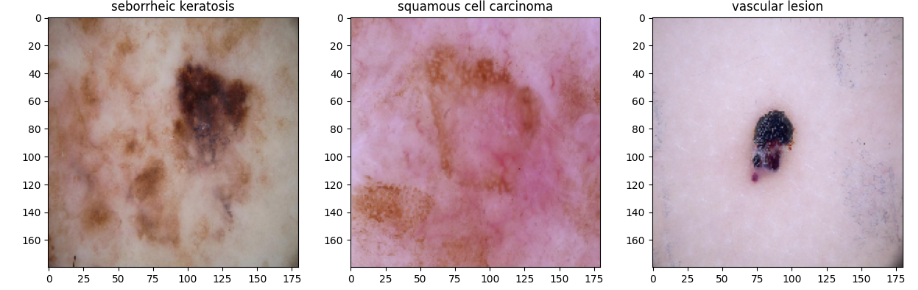
\includegraphics[width=0.45\textwidth]{derry.png}
  \caption{Sample dataset with their class labels}
  \label{fig: Sample dataset}
\end{figure}

\begin{figure}[H]
  \centering
  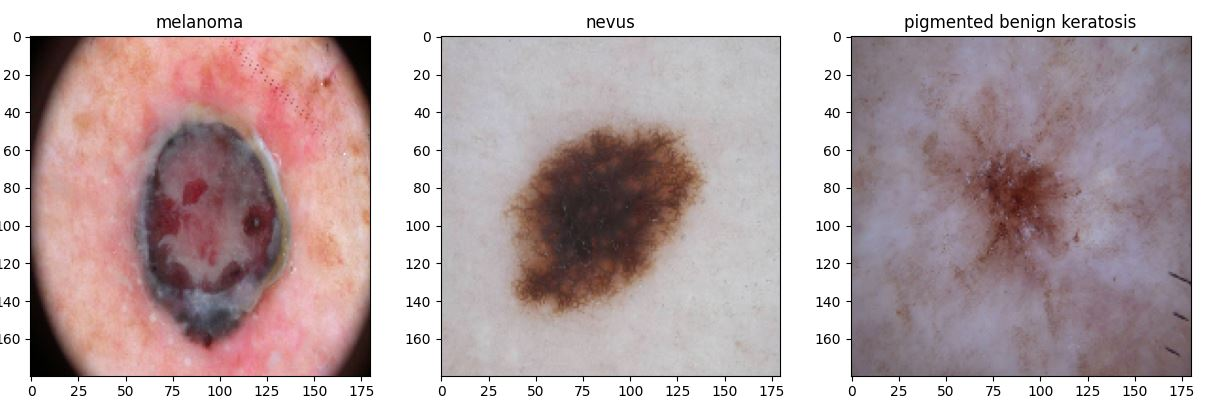
\includegraphics[width=0.45\textwidth]{dataset.jpg}
  \caption{Sample dataset with their class labels}
  \label{fig: Sample dataset}
\end{figure}

\section{SECTION 3}

\subsection{Proposed Approach}
The proposed approach involves preprocessing of the skin lesion images followed by feature extraction and classification. The preprocessing step involves noise removal and enhancement of the image contrast using histogram equalization.

\subsection{Pre-processing}
Holistically, during the preprocessing, noise removal, contrast enhancement, image resizing, rotation and zooming, and intensity are some of the inexhaustible techniques applied to extract and detect lesions efficiently in subsequent stages.  Loss balancing has been applied to overcome class imbalance for the multi-class skin lesion classification in the dataset. Convolutional Neural Network (CNN) based algorithms indicate their ability to extract and learn desired deep features from the input images and yield results with high performance. That said this algorithm will be implored to train, test and create the model for the detection of various cancerous skin.

\subsection{Methodology}
CNNs are neural networks with specific architectures that are prominent in areas such as image classification and recognition. They can be used to identify faces, objects, and traffic signs far better than humans. CNN is incorporated into robots and self-driving cars. They are supervised learning methodology that is trainable data labeled with respect to classes. 
In recent times, automatic skin lesion detection with CNNs has proven to be very efficient with higher performance. These algorithms have shown their ability to extract and learn appropriate deep features from the training images. The main goal of the paper is to evaluate and implement a CNN algorithm with image processing techniques for the automatic detection of skin cancer.
Essentially, CNNs learn the relation between the input object and the class labels. These compose of two components: the layer that performs the feature extraction and that which is used for the actual classification. 
CNN can be used to classify skin lesions in the following two ways: a CNN pre-trained on another large dataset, such as ImageNet can be applied as a feature extractor. With this, another classifier performs a classification, such as k-nearest neighbors, support vector machines, or artificial neural networks.  On the other way, a CNN can directly learn the relationship between the raw pixel data and the class label through end-to-end learning. Therefore, the latter is what this paper intends to explore. For a successful training of deep CNN models, the basic requirement is sufficient training data labeled with the classes available. And a highly optimized computer system with sufficient resources.

\begin{figure}[H]
  \centering
  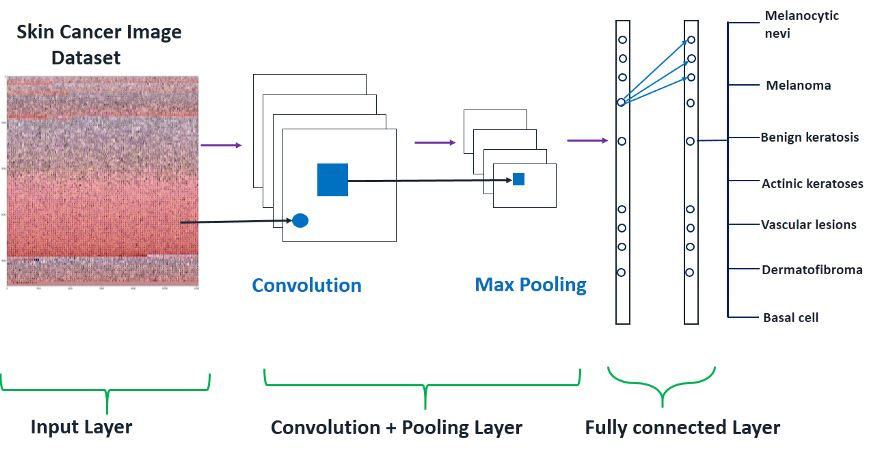
\includegraphics[width=0.45\textwidth]{modelArchetect.jpg}
  \caption{The CNN Architecture}
  \label{fig:image}
\end{figure}

In the fully connected layer, the options are to fine-tune all layers of the CNN or the front layers can be frozen just because of overfitting problems.
Extracted textural features are energy, homogeneity, entropy, contrast, correlation, cluster shade
prominence, variance information, a measure of correlation, and dissimilarity. The image is pre-processed by using the maxpooling filter for feature extraction which helps to maintain the intensity of the image.
An augmentor also known as a data augmentor or image augmentor, is used to increase the size and diversity of the training dataset. Moreover, this helped to generate new images with some variations of the original image. It helps to transform and modify the original data by changing the brightness, contrast, color saturation, rotation, scaling, flipping, and cropping the images.
For the data augmentation, I choose to: Randomly rotate some training images by 10 degrees Randomly Zoom by 10\% some training images. Randomly shift images horizontally by 10\% of the width. Randomly shift images vertically by 10\% of the height Once our model is ready, we fit the training dataset. It helped improve the generalization and robustness of the machine learning model and reduced overfitting. 

\begin{figure}
  \centering
  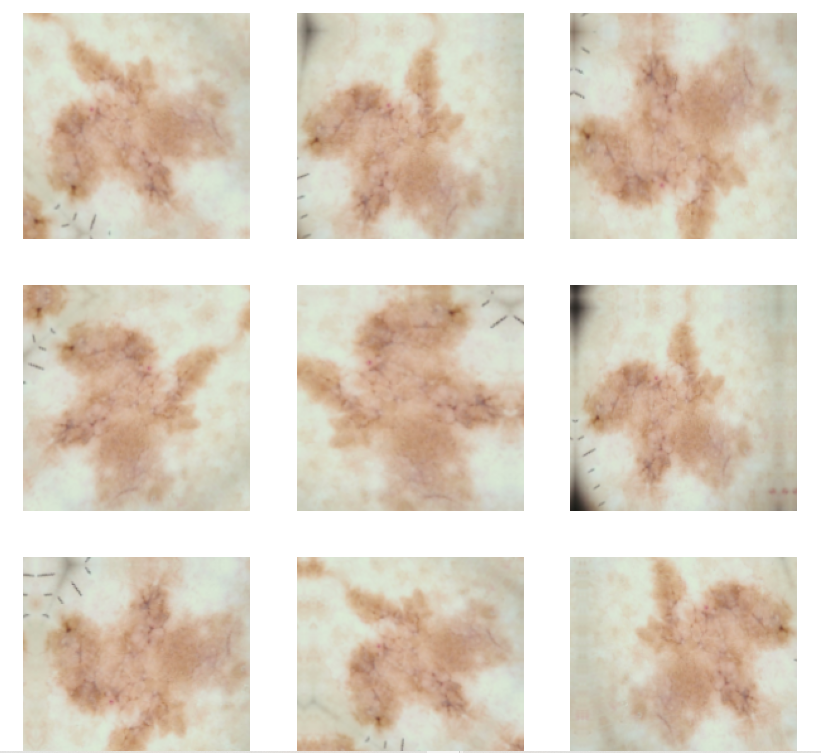
\includegraphics[width=0.45\textwidth]{augmented data.png}
  \caption{Data Argumnetation Image}
  \label{fig:image}
\end{figure}

Dropout is a regularization technique used in deep learning neural networks to prevent overfitting, which occurs when a model performs well on the training data but poorly on the testing data or new unseen data.
During training, each neuron in a dropout layer has a probability of being dropped out or deactivated randomly in a layer during training which is typically set to a small value between 0.1 and 0.5.  This methodology was employed to improve the model performance.

These forces other neurons in the network to learn more robust and generalizable features.
The dropout layer is inserted between the fully connected layers of the neural network, and the input to the dropout layer is the output from the previous fully connected layer.
The noise removal is performed using a median filter, which is effective in removing salt-and-pepper noise commonly present in medical images. 

The rotation and resizing are performed using a built-in function augment which accepts parameters useful to enhance the image by redistributing the pixel intensity values. 
I used the Keras Sequential API, where you have to add one layer at a time, starting from the input. The first is the convolutional (Conv2D) layer. It is like a set of learnable filters. I chose to set 32 filters for the two first conv2D layers and 64 filters for the two last ones. Each filter transforms a part of the image (defined by the kernel size) using the kernel filter. The kernel filter matrix is applied to the whole image. Filters can be seen as a transformation of the image. The CNN can isolate features that are useful everywhere from these feature maps or image transformations.
The second important layer in CNN is the pooling (MaxPool2D) layer. This layer simply acts as a down-sampling filter. It looks at the 2 neighboring pixels and picks the maximal value. Which are used to reduce the computational cost, and to some extent also reduce overfitting. 
Combining convolutional and pooling layers, CNN is able to combine local features and learn more global features of the image.
'relu' is the rectifier (activation function max(0,x). The rectifier activation function is used to add nonlinearity to the network.
The Flatten layer is used to convert the final feature maps into a single one-dimensional vector. This is useful as it is needed to make use of fully connected layers after some convolutional/max pool layers. It combines all the found local features of the previous convolutional layers.

% Define variables
\newcommand{\grad}{\nabla_\theta L(\theta)}
\newcommand{\mt}{m_t}
\newcommand{\vt}{v_t}
\newcommand{\mhat}{\hat{m}_t}
\newcommand{\vhat}{\hat{v}_t}
\newcommand{\eps}{\epsilon}
\newcommand{\lr}{\alpha}
\newcommand{\betaone}{\beta_1}
\newcommand{\betatwo}{\beta_2}

\subsection{The ADAM Optimizer}
In all instances of the compiling process, I used the ADAM optimization function which works by computing adaptive learning rates for each parameter based on estimates of the first and second moments of the gradients.\cite{reddi2019convergence} The first instant represents the mean of the gradient, while the second moment is the gradient variance. This causes the algorithm to converge to the minimum quickly.
It works by computing the gradient of the loss function with the given parameters. \cite{kingma2014method} In succession, it as well computes the first-moment estimate of the gradient and the second-moment estimate of the gradient. And in the end, it finds the bias-corrected estimates of the first and second moments. Not the  is a small constant added for numerical stability.


% Compute first moment estimate
\[\mt = \betaone\mt-1 + (1-\betaone)\grad\]

% Compute second moment estimate
\[\vt = \betatwo\vt-1 + (1-\betatwo)\grad^2\]

% Compute bias-corrected estimates
\[\mhat = \frac{\mt}{1-\betaone^t}\]
\[\vhat = \frac{\vt}{1-\betatwo^t}\]

% Update parameters
\[\theta_{t+1} = \theta_t - \lr\frac{\mhat}{\sqrt{\vhat} + \eps}\]

Although the ADAM optimizer can converge to a non-stationary point under certain conditions.\cite{ruder2016overview} Such as a point where the first and second moments of the gradients are equal, which might not be a local minimum of the loss function. For this term paper, I found it appropriate due to its fast convergence, and robustness to noisy or sparse gradients.

\subsection{The relu Activation Function}
The Relu(Rectified Linear Unit) Activation Function
During the creation of each of the CNN architecture, I used the relu activation function, due to the effectiveness of its derivative which is important for backpropagation thus helping to update the weights during training. Moreover, it helps the model learn complex patterns and capture the relationships between features in the data.

Below is the Relu equation:\\

\( \text{ReLU}(x) = \max(0, x) \)

\[
\text{ReLU}(x) = 
\begin{cases}
0, & \text{if}\ x \leq 0 \\
x, & \text{if}\ x > 0
\end{cases}
\]


x is the input value in this equation. Depending on which is larger, the function will either return 0 or x. This indicates that the function returns x if x is positive and returns 0 if x is negative or zero.


\begin{figure}[H]
  \centering
  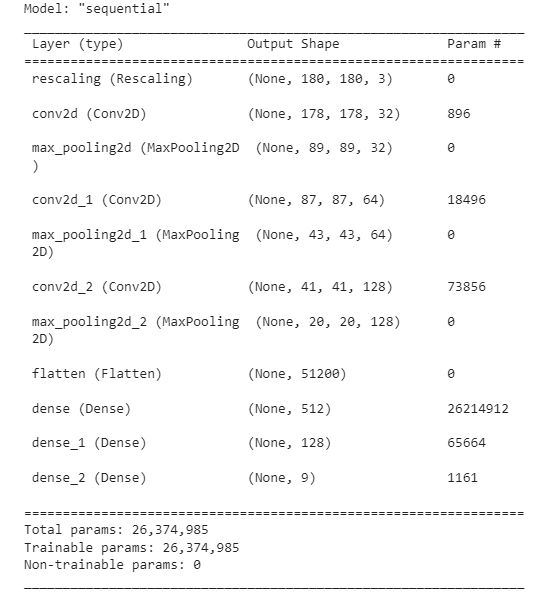
\includegraphics[width=0.45\textwidth]{modelsequence.jpg}
  \caption{Model Summary}
  \label{fig:image}
\end{figure}
\raggedbottom

\section{SECTION 4}
\subsection{Results}
The high accuracy, precision, and recall values indicate that the CNN model performs well in detecting skin cancer and distinguishing it from benign skin lesions. The F1-score, which is a harmonic mean of precision and recall, also supports this conclusion 
The CNN-based skin cancer detection model demonstrated strong performance in accurately identifying skin cancer. The high accuracy and precision values indicate that the model has the potential to be a valuable tool in assisting dermatologists in Ghana. Future work should focus on further refining the model's performance, expanding the dataset to include more diverse skin types and cancer stages, and integrating the model into a user-friendly platform for seamless adoption by dermatologists. Most importantly with higher computational powers, the epoch could be autotuned to a higher value to further increase the accuracy and precision. 
\begin{figure}[H]
  \centering
  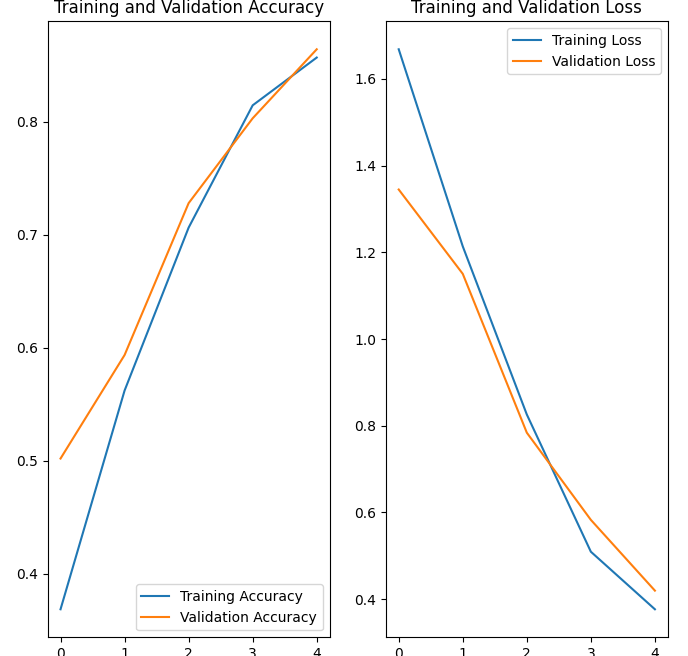
\includegraphics[width=0.45\textwidth]{trainloss.png}
  \caption{Training and Validation accuracy Vrs Training and Loss}
  \label{fig:image}
\end{figure}
\raggedbottom





\section{SECTION 5}
\subsection{Conclusion}
In conclusion, it seems the model has a maximum number of incorrect predictions for Basal cell carcinoma which has code 3, then the second most misclassified type is Vascular lesions code 5 then Melanocytic nevi code 0 whereas Actinic keratoses code 4 has the least misclassified type.
We can also further tune our model to easily achieve an accuracy above 80\% and I think still this model is efficient in comparison to detection with human eyes having 77.0344\% accuracy.
Convolutional neural networks have demonstrated considerable promise for helping dermatologists identify skin cancer. Due to low computational resources, I had to rely on a few epochs and fewer datasets to run the model. However, for an effective and better accuracy of the model, the incorporation of additional datasets and a well-resourced computer would help increase diagnostic precision and accuracy.



\bibliographystyle{apalike}
\bibliography{ref.bib}





\end{document}